% --------------------------------------------------------------------------
% Report template for BIR projects
% Report template with support for Portuguese and English languages
% Change language {brazil or english} in \documentclass as per the examples
% This template has support for the ABNT citing format
% 
% Original version: jan/2019
% https://github.com/
% 
% Based on ABNTEX2 and the thesis template
% --------------------------------------------------------------------------
\documentclass[
%\DeclareUnicodeCharacter{200B}{}
% --------------------------------------------------------------------------
% classe memoir . options                                                   
12pt,					% tamanho da fonte
openright,				% cap. começam em pág ímpar (ins pág vazia caso preciso)
twoside,				% para impressão em verso e anverso. Oposto a oneside
a4paper,				% tamanho do papel
% --------------------------------------------------------------------------
% classe abntex2 . options                                                  
%chapter=TITLE,			% títulos de capítulos convertidos em letras maiúsc.
%section=TITLE,			% títulos de seções convertidos em letras maiúsc.
%subsection=TITLE,		% títulos de subseções convertidos em letras maiúsc.
%subsubsection=TITLE,	% títulos de subsubseções convertidos em letras maiúsc.
% --------------------------------------------------------------------------
% Opções de IDIOMA do pacote babel                                          
english,
brazil
]{ABNT/abntex2_report}
% --------------------------------------------------------------------------
% Pacotes básicos    
\usepackage{lmodern}			% Usa a fonte Latin Modern			
\usepackage[T1]{fontenc}		% Selecao de codigos de fonte.
\usepackage[utf8]{inputenc}		% Codificacao do documento (conversão automática dos acentos)
\usepackage{indentfirst}		% Indenta o primeiro parágrafo de cada seção.
\usepackage{color}				% Controle das cores
\usepackage{graphicx}			% Inclusão de gráficos
\usepackage{microtype} 			% para melhorias de justificação
\usepackage{lipsum}	
\usepackage[brazilian,hyperpageref]{backref} % páginas com citações na bibliog.
%\usepackage[alf,abnt-etal-list=0,abnt-etal-cite=3,abnt-emphasize=bf]{abntex2cite}
\usepackage[alf]{abntex2cite}
%	
\usepackage{lastpage}			% Usado pela Ficha catalográfica
%\usepackage{subfig}
\usepackage{supertabular}       % tabela na capa do documento
\usepackage{booktabs}
\usepackage[table,xcdraw]{xcolor}
\usepackage{adjustbox}
\usepackage{amssymb,amsmath,mathrsfs}
\usepackage{algorithm,algpseudocode}
\usepackage{pgfplots}
\usepackage{tikz}
\usepackage{titlesec}
\usepackage{ragged2e}
\usepackage{tocloft}
\usepackage{threeparttable}
\usepackage{etoolbox}
\usepackage[normalem]{ulem}
\usepackage{yaacro}
\usepackage[none]{verlab}
%\usepackage{fontspec}
%\setmainfont{Helvetica Light}
\usepackage{lscape}
%\usepackage[graphicx]{realboxes}
\usepackage{rotating}
\usepackage{wrapfig}
\usepackage{caption}
\usepackage{subcaption}
\usepackage{dirtytalk}
\usepackage{pdfpages}
\usepackage{threeparttable}
\usepackage{hyperref}
%\hypersetup{draft}
\usepackage{float}
\DeclareUnicodeCharacter{200B}{}
% --------------------------------------------------------------------------%
% Configurações do PDF final                                                
\definecolor{blue}{RGB}{41,5,195}
\makeatletter
\hypersetup{
	%pagebackref=true,
	pdftitle={\@title}, 
	pdfauthor={\@author},
	pdfsubject={\@title},
	%pdfsubject={\imprimirpreambulo},
	pdfcreator={LaTeX with abnTeX2},
	pdfkeywords={abnt}{latex}{abntex}{abntex2}{\imprimirpalavraschave}, 
	colorlinks=true,       		% false: boxed links; true: colored links
	linkcolor=blue,          	% color of internal links
	citecolor=blue,        		% color of links to bibliography
	filecolor=magenta,      	% color of file links
	urlcolor=blue,
	bookmarksdepth=4
}
%\makeatother
% --------------------------------------------------------------------------
% Posiciona figuras e tabelas no topo da página quando adicionadas sozinhas
% em um página em branco. Ver https://github.com/abntex/abntex2/issues/170
%\makeatletter
\setlength{\@fptop}{5pt} % Set distance from top of page to first float
\makeatother
% --------------------------------------------------------------------------
% Formatação                                                                
\newcommand\tab[1][1cm]{\hspace*{#1}}
\apptocmd{\thebibliography}{\justifying}{}{} 
\renewcommand{\ABNTEXsectionfont}{\bfseries}
\titlespacing*{\chapter}{0pt}{0pt}{12pt}
\titlespacing*{\section}{0pt}{6pt}{6pt}
\titlespacing*{\subsection}{0pt}{6pt}{6pt}
\titlespacing*{\subsubsection}{0pt}{6pt}{6pt}
% --------------------------------------------------------------------------
% Rearranja os finais de cada estrutura                                     
\algrenewtext{EndWhile}{\algorithmicend\ \algorithmicwhile}
\algrenewtext{EndFor}{\algorithmicend\ \algorithmicfor}
\algrenewtext{EndIf}{\algorithmicend\ \algorithmicif}
\algrenewtext{EndFunction}{\algorithmicend\ \algorithmicfunction}
% --------------------------------------------------------------------------
% Espaçamentos entre linhas e parágrafos                                    
\setlength{\parindent}{1.3cm} % linha
\setlength{\parskip}{0.2cm} % parágrafo, tente também \onelineskip
% --------------------------------------------------------------------------
% Informações de dados para CAPA e FOLHA DE ROSTO                           
\prodtecnica{001 / 2020}
\titulo{Aplicações Práticas da SunBurn}
\tiporelatorio{Final} 
\nomeprojeto{Sistemas Produtivos}
\outrossubtitulos{~} % opcional
\autores{
	Jéssica Lima Motta\\
	Leonardo Mendes de Souza Lima\\
	Vinícius José Gomes de Araujo Felismino\\
	Pedro Paulo Ventura Tecchio\
}
% \newcommand{\autoresexternos}{
% 	John Marston\\
% 	Frank West\
% }
\local{Salvador\\Bahia, Brasil}
\data{Setembro de 2020}
% \classificacao{( ) Confidencial  (X) Restrito  ( )  Uso Interno  ( ) Público}
% \revisao{01}
% \tabelacutter{000} 
% \palavraschave{1. Manipulator. 2. Simulation. 3. Computer vision.}
% \classificacaoassunto{000} % sNúmero de Classificação do assunto 
%\parceirologo{logos/x.png}
%------------------------------------------------------------------
% Finalização das configurações da capa
%
%
%------------------------------------------------------------------              
% Acrônimos :: Chamar no texto como \ac{DoF}                                
% \begin{acgroupdef}[list=acronyms]
% 	\acdef{DoF}{Degrees of Freedom}
% 	\acdef{PoC}{Proof of Concept, em português Prova de Conceito}
% 	\acdef{UUV}{Unmanned Underwater Vehicle, em português Veículo Subaquático Não-tripulado}
% 	\acdef{AUV}{Autonomous Underwater Vehicle, em português Veículo Subaquático Autônomo}
% 	\acdef{UVM}{Unmanned Vehicle Morphing}
% 	\acdef{SLAM}{Simultaneous Localization and Mapping}
% 	\acdef{ROV}{Remotely Operated Vehicle}
% 	\acdef{SOTA}{Study Of The Art}
% 	%
% 	%
% 	%
% \end{acgroupdef}
% --------------------------------------------------------------------------
% Criação do sumário
\makeindex
%
\begin{document}
	% \frenchspacing
	\imprimircapa
	% \imprimircatalografica
% --------------------------------------------------------------------------
% Sumário executivo                                                         
	% \ABNTEXchapterfont\large\textbf{\execsummarytitlename}
	% \begin{flushleft}
	% 	\normalsize
	% 	\justify
	% 	\normalfont
	% 	O projeto de Manipuladores - Desafio.2, também conhecido como \textbf{xxxxx} se configura sob o Programa de Formação de Novos Talentos do Serviço Nacional de Aprendizagem Industrial, Departamento Regional da Bahia - Senai/DR/BA, sendo este o principal fomentador do programa.

	% 	O projeto foi considerado como início técnico do projeto o dia 00 de bolsoneiro de 2020. 

	% 	O prazo de execução planejado é de xx meses.
	% \end{flushleft}
	% \clearpage
%------------------------------------------------------------------
% Resumo e abstract                                                         
	\ABNTEXchapterfont\large\textbf{\resumoatitlename}
	\begin{flushleft}
		\normalsize
		\justify
		\normalfont
		%resumo aqui
		%
		%
		%
	\end{flushleft}
	% \vspace*{1cm}
	% \newpage
	% %
	% \ABNTEXchapterfont\large\textbf{\resumobtitlename}
	% \begin{flushleft}
	% 	\normalsize
	% 	\justify
	% 	\normalfont
	% 	%abstract aqui
	% 	%
	% 	%
	% 	%
	% \end{flushleft}
	% \clearpage
% --------------------------------------------------------------------------
% Lista de figuras                                                          
	% \begin{flushleft}
	% 	\ABNTEXchapterfont\Large\textbf{\MakeUppercase\listadefigurasname}
	% \end{flushleft}
	% \vspace*{-36pt}
	% \pdfbookmark[0]{\listfigurename}{lof}
	% \normalsize
	% \listoffigures*
	% \cleardoublepage
% --------------------------------------------------------------------------
% Lista de tabelas                                                          
	% \begin{flushleft}
	% 	\ABNTEXchapterfont\Large\textbf{\MakeUppercase\listadetabelasname}
	% \end{flushleft}
	% \vspace*{-36pt}
	% \pdfbookmark[0]{\listtablename}{lot}
	% \normalsize
	% \listoftables*
	% \cleardoublepage
% --------------------------------------------------------------------------
% Lista de símbolos e abreviaturas                                          
	% \begin{flushleft}
	% \ABNTEXchapterfont\Large\textbf{\MakeUppercase\listadesimbolsabrevtitlename}
	% 	\noindent
	% 	\vspace*{-06pt}
	% 	\pdfbookmark[0]{\listadesiglasname}{lot}
	% 	\normalsize
	% 	\normalfont
	% 	\aclist[list=acronyms]
	% \end{flushleft}
	% \newpage
% --------------------------------------------------------------------------
% Tabela de conteúdo                                                        	
	% \begin{flushleft}
	% 	\ABNTEXchapterfont\Large\textbf{\MakeUppercase\glosariotitlename}
	% \end{flushleft}
	% %\pagebreak
	% \vspace*{-36pt}
	% \pdfbookmark[0]{\contentsname}{toc}
	% \normalsize
	% \normalfont
	% \tableofcontents*
	% \justify
% --------------------------------------------------------------------------
% Formatação, remover espaço depois dos títulos
	\setlength\beforechapskip{-24pt}
	\setlength\afterchapskip{12pt}
	\textual
	\pagestyle{plain}
	\normalsize
	\justify
	\normalfont
% --------------------------------------------------------------------------
% Conteúdo do relatório  
	\chapter{INTRODUÇÃO}
\label{chap:intro}
Como parte da etapa de desenvolvimento do projeto de Automação de Operações com \textit{\acs{ROV}}, \cite{pybullet}

\cite{sivvcev2018underwater}

Entretanto

%------------------------------------------------------------------
\section{Objetivos}
\label{sec:obj}
Projetar e construir uma prova de conceito para subsidiar a análise de viabilidade técnica-econômica de automatizar operações submarinas com manipuladores de \textit{\acs{ROV}}, também conhecido como veículo submarino operado remotamente.


%------------------------------------------------------------------
\section{Justificativa} %motivação
\label{sec:just}
Nesta etapa da automação de um manipulador, 


%------------------------------------------------------------------
\section{Organização do relatório}
\label{sec:org}
Este documento está organizado da seguinte forma, o capítulo 

%----------------------- marcado
\section{Resumo da empresa}
\label{sec:rese}
A SunBurn é uma empresa de nome fictício que atua no desenvolvimento, implantação e operação de projetos de energia renovável. No Brasil, é sediada no sul do país e opera nas regiões Norte, Sul e Nordeste.

Os projetos da empresa, nos Ambientes de Contratação Regulada (ACR) e Contratação Livre (ACL), somam 642 Megawatts de potência vendida. Todos os empreendimentos são monitorados à distância por meio do Centro de Operações localizado na sede da SunBurn, na região Sul.
A SunBurn estabelece um modelo de negócios com maior segurança e rentabilidade a seus investidores, mantendo o compromisso de fornecer energia limpa e confiável.

Os empreendimentos têm como característica fundamental a qualidade, apresentando altos fatores de capacidade e geração garantida. Aliado ao modelo de gestão da SunBurn, que segue os princípios do ESG (Environmental, Social and Corporate Governance), a alta tecnologia e profissionais qualificados garantem confiabilidade na operação.

A sustentabilidade é fator indissociável da estratégia de negócios da SunBurn. Nas regiões onde a empresa atua, as operações têm foco na redução de impactos ambientais, no desenvolvimento das comunidades da região e na segurança dos colaboradores.





	% \chapter{PACOTE DE VALOR}
\label{chap:pacotedevalor}

O pacote de valor é definido como sendo um conjunto de bens e serviços fornecidos, em variadas proporções, para os clientes. Desta forma as empresas que prestam serviços ou fornecem produtos passam a fornecer outros itens que agregam e consolidam as relações com seus clientes.
Apesar do pacote de valor fortalecer essas relações é necessário que as empresas expandam os mesmos fornecendo mais benefícios aos clientes.
Para se produzir o pacote de valor o processo é semelhante à produção de produto, como descrito na Figura \ref{fig:pacotevalor}.

\begin{figure}[H]
    \caption{Fluxo da geração do pacote de valor.}
    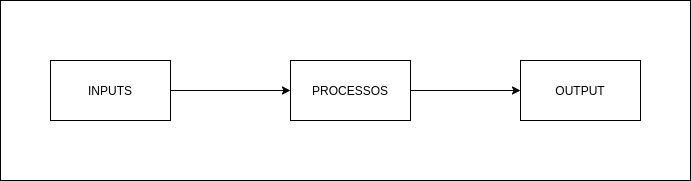
\includegraphics[width=\textwidth]{images/pacote_valor.png}
    \label{fig:pacotevalor}
    \caption*{Fonte: baseado no Slack, 2006.}

\end{figure}

Os inputs podem ser divididos em: recursos a serem transformados (matérias-primas, informações e clientes) ou recursos de transformação (instalações e prédios, máquinas e equipamentos, e empregados). Os processos englobam o projeto, planejamento e controle, melhorias e estratégias de produção. E como output tem-se os bens e serviços, ou seja, o pacote de valor \cite{slack2006administraccao}.
%------------------------------------------------------------------
\section{Aplicação Prática}
\label{sec:app1}
O pacote de valor da empresa SunBurn revolve entorno da produção e venda de energia elétrica, bem como serviços agregados. No território nacional, esta empresa produz energia elétrica através da produção solar e eólica, a qual é fornecida para empresa distribuidora regionalmente instalada. 

Acredita-se que o pacote de valor da empresa pode ser expandido através da integração das tecnologias de produção de forma que ela possa garantir o fornecimento da energia que vende mesmo quando algum incidente ocorra na geração através de uma das tecnologias. O atual uso de diferentes fontes limpas de energia aumenta deve apenas ser realizado de forma integrada de forma a criar uma redundância do sistema de produção da Sunburn. Esta integração pode então ser vendida como um serviço adicional de aumento na garantia da entrega de energia para o cliente.

A SunBurn já possui um estudo para a formação de micro-geradoras de energia elétrica, as quais são implantadas direto no cliente final. Tal modo de produção viabiliza a redução dos custos agregados na transmissão e distribuição de energia elétrica para o cliente, além de possibilitar uma redundância local no fornecimento de energia para o cliente em questão. Esse modo de geração de energia, poderá ser amplamente utilizado pela SunBurn após a regulamentação local da venda de energia elétrica produzida por essas micro-geradoras para as empresas de transmissão e distribuição. A SunBurn poderá oferecer os seus serviços de regulação, controle e manejo do fornecimento de energia para os seus clientes que possuam usinas micro-geradoras, de forma que os clientes possam vender o excedente de energia gerado em seus territórios.



% \subsection{Requisitos do cliente}
% \label{sub:reqc}

	% \chapter{SISTEMA PRODUTIVO}
\label{chap:desenv}


%------------------------------------------------------------------
\section{Descrição do sistema}
\label{sec:descsis}

\subsection{Arquitetura geral}
\label{sub:arqg}

\subsection{Especificação técnica}
\label{sub:esptec}

\subsection{Estrutura analítica do protótipo}
\label{sub:eap}



%------------------------------------------------------------------
\section{Especificação funcional} %na introdução da seção apresentar a conexão entre as funcionalidades
\label{sec:sota}



\subsection{Funcionalidade A}
\label{sub:funcA}
%aqui vc apresenta a funcionalidade

\subsubsection{Descrição} %incluir o fluxograma da funcionalidade aqui
\label{ssub:descA}

\subsubsection{Premissas necessárias}
\label{ssub:premA}

\subsubsection{Dependências}
\label{ssub:depA}

\subsubsection{Saídas}
\label{ssub:saidaA}



\subsection{Funcionalidade B}
\label{sub:funcB}

\subsubsection{Descrição} %incluir o fluxograma da funcionalidade aqui
\label{ssub:descB}

\subsubsection{Premissas necessárias}
\label{ssub:premB}

\subsubsection{Dependências}
\label{ssub:depB}

\subsubsection{Saídas}
\label{ssub:saidaB}


%------------------------------------------------------------------
\section{Arquitetura de software}
\label{sec:arqs}
%introdução ao assunto apresentando a arquitetura


\subsection{Diagrama de componentes}
\label{sub:diagcomp}


\subsection{Matriz de rastreabilidade de testes}
\label{sub:matrast}


%------------------------------------------------------------------
\section{Simulação do sistema}
\label{sec:simul}


\section{Integração}
\label{sec:integra}



\section{Testes realizados}
\label{sec:testes}









	% \chapter{RESULTADOS E ANÁLISES}
\label{chap:result}


%------------------------------------------------------------------
\section{Resultados alcançados}
\label{sec:resalcanc}


%------------------------------------------------------------------
\section{Análise dos experimentos}
\label{sec:doe}


%------------------------------------------------------------------
\section{Avaliação da prontidão tecnológica}
\label{sec:trl}



	% \chapter{CONFIABILIDADE DO SISTEMA}
\label{chap:conf}

%------------------------------------------------------------------
\section{Análise dos modos e efeitos de falhas}
\label{sec:fmeca}

%------------------------------------------------------------------
\section{Diagrama de blocos da Confiabilidade}
\label{sec:diag}

%------------------------------------------------------------------
\section{Análise da árvore de falhas}
\label{sec:fta}


	% \chapter{GESTÃO DO CONHECIMENTO}
\label{chap:conhec}

%------------------------------------------------------------------
\section{Lições aprendidas}
\label{sec:licap}

%------------------------------------------------------------------
\section{Guia de uso}
\label{sec:guia}


	% \chapter{CONCLUSÃO}
\label{chap:conclu}





	%\chapter{REFERENCIAL TEÓRICO}
\label{chap:refer}

%------------------------------------------------------------------
\section{Princípios de robótica}
\label{sec:princ}



	%\chapter{MATERIAIS E MÉTODOS}
\label{chap:metod}


%------------------------------------------------------------------
\section{Metodologia aplicada}
\label{sec:metaplic}




%------------------------------------------------------------------
\section{Especificação dos componentes utilizados} 
\label{sec:especif}



% --------------------------------------------------------------------------
% Referências
	% \cleardoublepage
	\titleformat{\chapter}[display]{\vspace*{-24pt}\ABNTEXchapterfont\large\bfseries}{\chaptertitlename\ \thechapter}{12pt}{\Large}
	\bibliography{bibliography}
% --------------------------------------------------------------------------
% Apêndices
	% \apendices
	% \justify
	% %
	% \chapter{Questões de abordagem à pesquisa}
	% \label{apend:quest}
	% %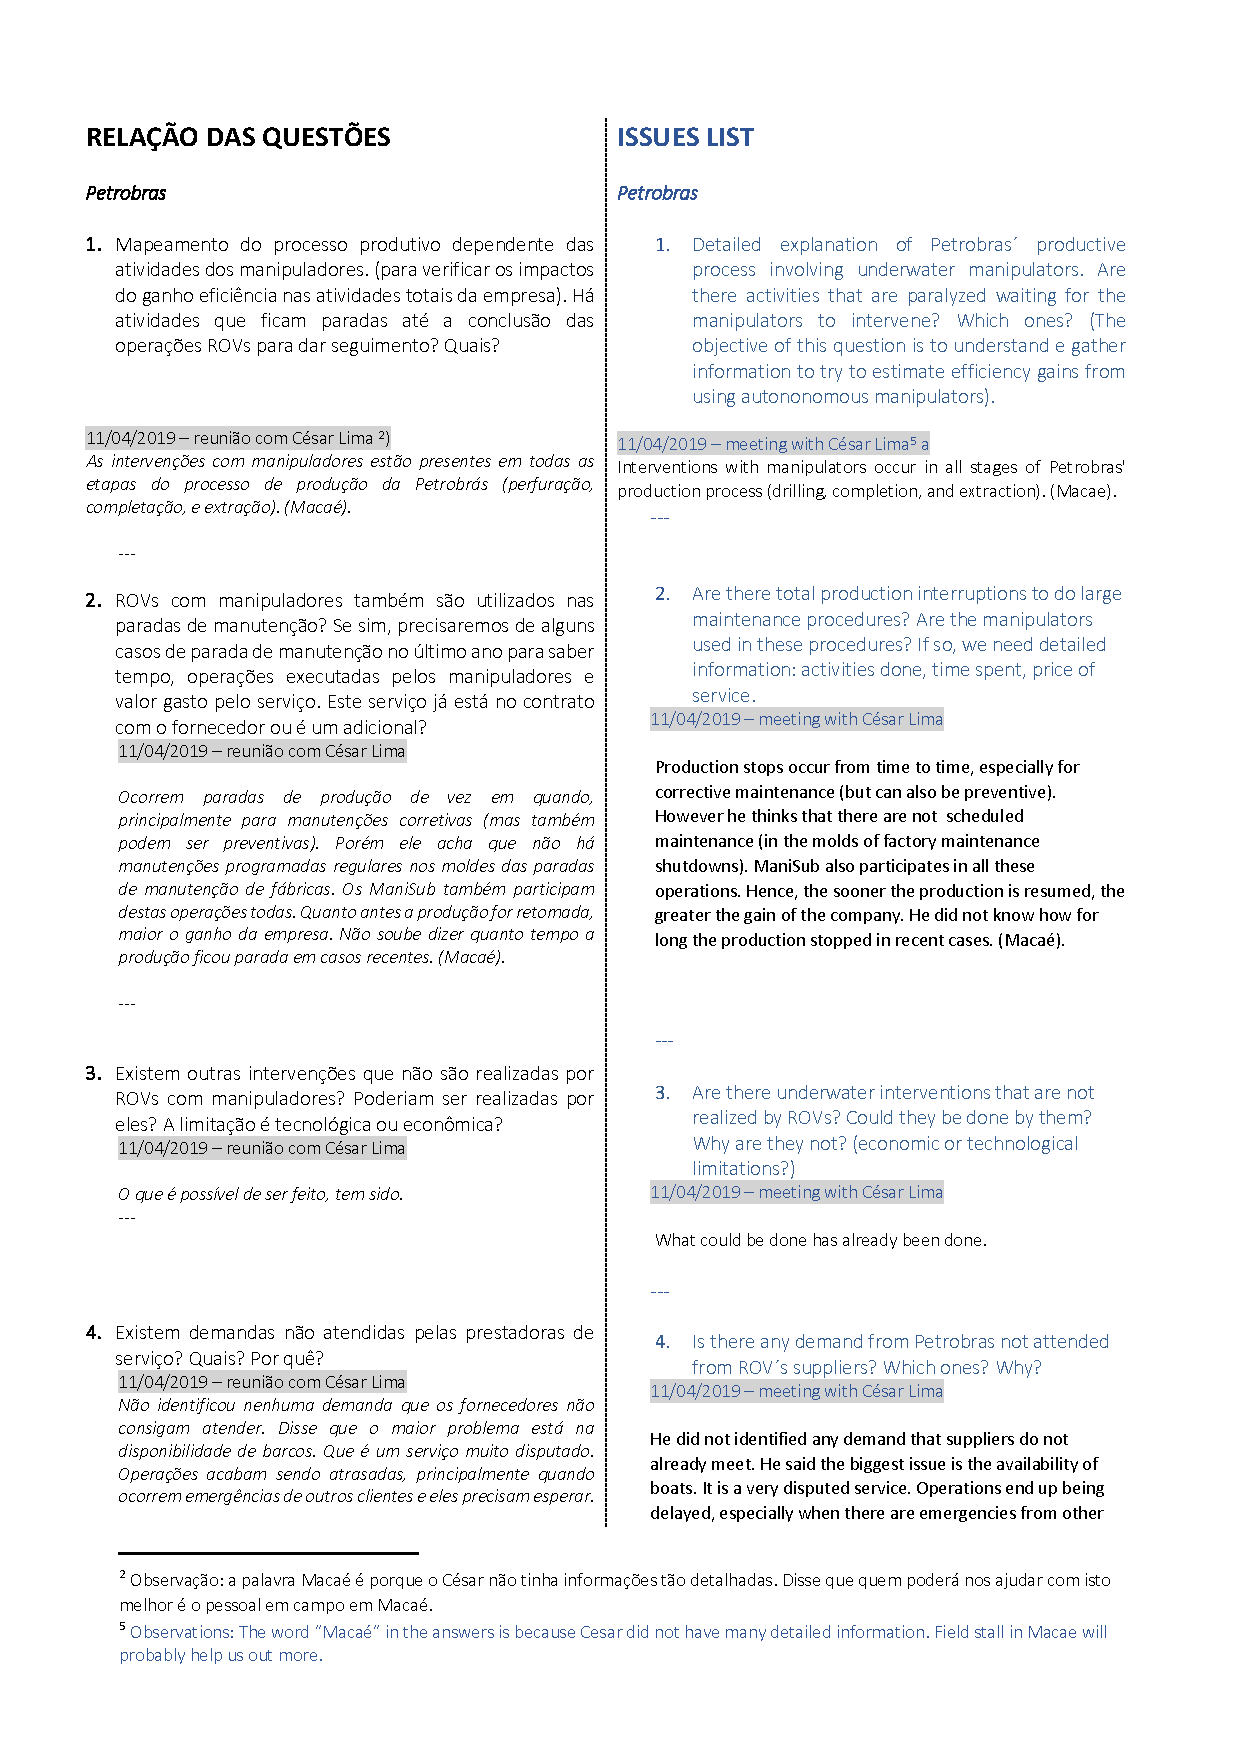
\includepdf[pages={{},-}]{appendix/listquest.pdf}
	% \lipsum[1] % Comentar e adicionar apêndice aqui
	% %
	% \chapter{Um assunto importante}
	% \label{apend:assunto}
	% \lipsum[1] % Comentar e adicionar apêndice aqui
	

% --------------------------------------------------------------------------
% % Anexos                                                                     
% 	\anexos
% 	\justify
% 	%
% 	\chapter{Outro assunto importante}
% 	\label{ann:relant}
% 	%\includepdf[pages={{},-}]{annex/manisubanterioridade.pdf}
% 	\lipsum[1] % Comentar e adicionar apêndice aqui
% 	%
\end{document} 